\chapter{Použité metody}

% korelace
% ortogonální
% kontingencni tabulka (vicenasobna)

% zkrtky PCA, MCA, CA,
% znaceni jendotkový vektor rozměru J \mathbf{1}_J
% Singulární rozklad (zkratkou SVD podle anglického názvu Singular Value Decomposition) matice + singulární hodnoty


\section{Redukce dimenzionality} %Extrakce proměnných}

\subsection{Analýza hlavních komponent}

Analýza hlavních komponent (anglicky \emph{Principal component analysis}, dále jako PCA) je statistická metoda využívaná pro pro extrakci proměnných, redukci vícedimenzio-\\nálních dat nebo vizualizaci dat. Lze ji aplikovat pouze na kvantitativní data s numerickými, spojitými hodnotami, neboť metoda využívá lineární algebraické techniky, jako je například kovarianční matice, pro jejíž výpočet se předpokládají spojité hodnoty. 

Jednotlivá pozorování obsažená v~datech bývají popsána několika různými příznaky. Tyto příznaky jsou často vzájemně korelované a obsahují šum. Metoda PCA dovede extrahovat pouze důležité informace z~proměnných a snížit šum. K~tomu je třeba vypočítat nové ortogonální proměnné, nazývané hlavní komponenty, které se získají jako lineární kombinace původních proměnných \cite{bib:PCA1}. Hlavní komponenty reprezentují směry největšího rozptylu původních dat a jsou řazeny podle své významnosti. Jinými slovy, první hlavní komponenta zachycuje co nejvíce variability v~datech, druhá hlavní komponenta zachycuje co nejvíce variability, která nebyla zachycena první hlavní komponentou, pro zbylé komponenty analogicky. \cite{bib:PCA3}
%, jinými slovy se jedná o přímku,  které nesou největší informaci o datech. Hlavní komponentu si lze představit jako novou osu, která umožňuje vidět data v~takovém rozložení, že rozdíly mezi pozorováními jsou lépe patrné.  %https://builtin.com/data-science/step-step-explanation-principal-component-analysis

\subsubsection{Princip}

Předpokládáme množinu dat $\mathbf{X} = (\bm{x}_1, \ldots, \bm{x}_N )$, kde $N$ j počet pozorování a každý vektor $\bm{x}_i$ přísluší jednomu pozorování popsanému $M$ proměnnými. $\mathbf{X}$ je potom matice rozměru $N\times M$ vstupních dat. Dále je definovaný výběrový průměr $\bar{\bm{x}}$ jako
\begin{equation}
    \bar{\bm{x}} = \frac{1}{N} \sum_{i=1}^{N} \bm{x}_i,
\end{equation}
a výběrová kovarianční matice $\mathbf{C}$

\begin{equation}
    \mathbf{\mathbf{C}} = \frac{1}{N} \sum_{i=1}^{N} (\bm{x}_i - \bar{\bm{x}}).
\end{equation}

První hlavní komponentu, která popisuje největší rozptyl dat označíme $y_{1i}$ a vypočteme následovně jako lineární kombinaci původních proměnných
\begin{equation}
    y_{1i} = \bm{a}_1^\top (\bm{x}_i - \bar{\bm{x}}), \quad \mbox{pro } i=1,\ldots,N,
\end{equation}
kde $\bm{a}_1 = (a_{11}, \ldots, a_{M1})^\top $ je vektor vah. 

Optimální vektor $\bm{a}_1$ je takový vektor, který maximalizuje výběrový rozptyl nové proměnné $y_{1i}$ za podmínky $\bm{a}_1^\top\bm{a}_1 = 1$. Pakliže je výběrový rozptyl $y_{1i}$ definován jako 
\begin{equation}
    D(y_{11}, \ldots, y_{1N}) = \bm{a}_1^\top \mathbf{C} \bm{a}_1
\end{equation}
můžeme maximalizační úlohu vyřešit pomocí metody Lagrangeových multiplikátorů. Lagrageova funkce s parametrem $\lambda_1$ má následující tvar
\begin{equation}
    \mathcal{L}(\bm{a}_1, \lambda_1) = \bm{a}_1^\top \mathbf{C} \bm{a}_1 - \lambda_1(\bm{a}_1^\top\bm{a}_1 - 1).
\end{equation}

Derivaci funkce položíme rovnou nule 
\begin{align*}
    \frac{\partial \mathcal{L}}{\partial \bm{a}_1}  = 2 \mathbf{C} \bm{a} - 2\lambda_1 \bm{a}_1 \overset{!}{=}  0 \\
    (\mathbf{C} - \lambda_1 \mathbf{I} ) \bm{a}_1 \overset{!}{=}  0,  \\
\end{align*}
kde $\mathbf{I}$ je jednotková matice.

Řešíme soustavu lineárních rovnic pro neznámý parametr $\bm{a}_1$, která má řešení právě tehdy, když je matice $\mathbf{C} - \lambda_1 \mathbf{I} $ singulární, tedy platí, že její determinant  je roven nule. $\lambda_1$ je pak největší vlastní číslo matice $\mathbf{C}$ a $\bm{a}_1$ vlastní vektor příslušný tomuto vlastnímu číslu. Toto tvrzení se matematicky zapíše následovně
\begin{equation}
    \mathbf{C} \bm{a}_1 = \lambda_1 \bm{a}_1. \\
\end{equation}
Po vynásobení vektorem $\bm{a}_1$ zleva získáme řešení pro maximální rozptyl proměnné $y_{1i}$
\begin{equation}
    D(y_{11}, \ldots, y_{1N}) = \bm{a}_1^\top \mathbf{C} \bm{a}_1 = \lambda_1.
\end{equation}


Druhá hlavní komponenta
\begin{equation}
    y_{2i} = \bm{a}_2^\top (\bm{x}_i - \bar{\bm{x}}), \quad \mbox{pro } i=1,\ldots,N,
\end{equation}
se vypočte obdobným způsobem s přidanou podmínkou ortogonality vzhledem~k první hlavní komponentě -- druhá hlavní komponenta nesmí být korelovaná s předchozí, první hlavní komponentou. Potom popisuje druhý největší možný rozptyl v~datech. Znázornění dvou hlavních komponent ve dvoudimenzionálním prostoru je vyobrazeno na obrázku \ref*{obr:met:PCA1}.
Vektor  $\bm{a}_2$ se opět získá jako jednotkový vlastní vektor kovarianční matice $\mathbf{C}$ příslušící druhému největšímu vlastnímu číslu $\lambda_2$.\cite{bib:PCA1, bib:PCA3} %https://builtin.com/data-science/step-step-explanation-principal-component-analysis

\begin{figure}[hbtp!]
    \centering
    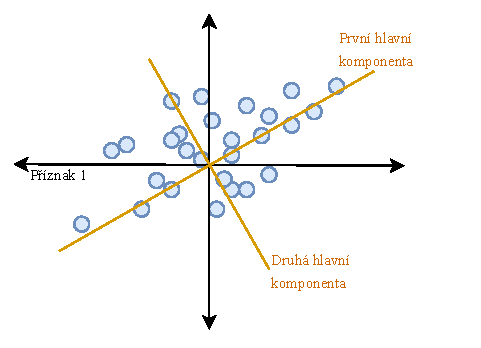
\includegraphics[width=0.7\textwidth]{obrazky/PCA.pdf}
    \caption{Znázornění dvou hlavních komponent na pro dvě proměnné. Zdroj: vlastní.}
    \label{obr:met:PCA1}
\end{figure}

Získání předpisů pro další hlavní komponenty je analogické. Obecně lze zapsat metodu PCA a převod původních proměnných následujícím maticovým zápisem
\begin{equation}
    \mathbf{Y} = \mathbf{XA}, 
\end{equation}
kde $\mathbf{Y}$ obsahuje komponenty $\bm{y}_{1}, \bm{y}_{2}, \ldots$, $\mathbf{X}$ je matice vstupních dat, $\mathbf{A}$ je matice vlastních vektorů kovarianční matice $\mathbf{C}$. Pro matici $\mathbf{A}$ zároveň platí $\mathbf{C} =  \mathbf{A} \mathbf{\Lambda} \mathbf{A}^\top$, kde $\mathbf{\Lambda}$ je diagonální matice vlastních čísel $\mathbf{C}$.\cite{bib:PCA2}

\subsection{Korespondenční analýza}

Vícenásobná korespondenční analýza (anglicky \emph{Multiple correspondence analysis}, dále jako MCA) je metoda, která umožňuje popsat vztahy mezi daty, které jsou popsané kategorickými proměnnými, vytvořením kontingenční tabulky. V případě, že se popisuje vzájemná relace pouze dvou proměnných, se použije základní korespondenční analýza\footnote{anglicky \emph{correspondence analysis} (CA)}. MCA je alternativou~k PCA, pokud jsou analyzovanými daty kategorická data. \cite{bib:MCA1}

% \subsubsection{Princip korespondenční analýzy}
\subsubsection{Značení}
%https://statmath.wu.ac.at/courses/CAandRelMeth/caipA.pdf
Nechť $\mathbf{N}$ je matice dat s rozměry $I\times J$, kde I odpovídá počtu pozorování a J je počet kategorií. %asi pocet kategorii, najit !!!
Matice $\mathbf{N}$ je převedena na korespondenční matici $\mathbf{P}$ vydělením matice $\mathbf{N}$ jejím celkovým součtem $n = \sum_{i=1}^{I} \sum_{j=1}^{J} n_{ij}=\mathbf{1}^\top_I \mathbf{N}\mathbf{1}_J$. To zaručuje, že součet prvků matice $\mathbf{P}$ je roven jedné. Tyto kroky lze shrnout následujícím matematickým zápisem
\begin{equation}
    \mathbf{P} = \frac{1}{n}\mathbf{N}, \qquad \mathbf{P} = \{p_{ij}\},  \qquad  \sum_{i=1}^{I} \sum_{j=1}^{J} p_{ij} = 1.
\end{equation}
Součet $i$tého řádku, resp. součet $j$tého sloupce je značen následovně
\begin{align*}
    r_i = \sum_{j=1}^{J} \qquad \mbox{ pro } i=1,\ldots,I, \\
    c_j = \sum_{i=1}^{I} \qquad \mbox{ pro } j=1,\ldots,J.
\end{align*}
Vektor $\bm{r} = \mathbf{P} \mathbf{1}_J $ obsahuje všechny řádkové součty matice $\mathbf{P}$, analogicky vektor $\bm{c} = \mathbf{P}^\top \mathbf{1}_I $ obsahuje všechny sloupcové součty téže matice.

Pro další výpočty zavedeme značení pro diagonální matice, které mají na diagonále  řádkový, resp. sloupcový součet
\begin{equation}
    \mathbf{D}_r = \mbox{diag}(\bm{r}), \quad \mbox{ resp. } \quad \mathbf{D}_c = \mbox{diag}(\bm{c}).
\end{equation}

% Pro připomenutí je vhodné dodat, že součet matice P je jedna

\subsubsection[Výpočetní algoritmus základní korespondeční analýzy]{Výpočetní algoritmus základní korespondeční analýzy \cite{bib:CA1,bib:MCA2}}
Označme $\mathbf{S}  = \{s_{ij}\}$ následující matici
\begin{equation}
    \mathbf{S} := \mathbf{D}_r^{-\frac{1}{2}} (\mathbf{P} - \bm{rc}^\top) \mathbf{D}_c^{-\frac{1}{2}}.
\end{equation}
Po té proveďme singulární rozklad této matice
\begin{equation}
    \mathbf{S} = \mathbf{U}\mathbf{\Delta}\mathbf{V}^\top,
\end{equation}
kde $\mathbf{\Lambda} = \mathbf{\Delta}^2$ je matice vlastních čísel $\lambda_k$ pro $k=1,\ldots,K$, kde $K=min\{I-1,J-1\}$. Potom rozměry matice $\mathbf{U}$, resp. $\mathbf{V}$ jsou $I\times k$, resp.  $J\times k$. Dále platí $\mathbf{U}^\top\mathbf{U}=\mathbf{V}^\top\mathbf{V}=\mathbf{I}$.%https://www.wikiwand.com/en/Correspondence_analysis


% Zatímco u PCA je měřítkem úspěchu míra rozptylu popsaná prvními vybranými hlavními komponentami 
Korespondenční analýza měří míru váženého rozptylu, tzv. inercii pomocí vlastních čísel $\lambda_k$ matice $\mathbf{S}$, $\lambda_k$ se pak nazývají hlavní inercie.
Celková inercie je rovna
\begin{equation}
    I = \sum_{k=1}^{K} \lambda_k = \sum_{i=1}^{I}\sum_{j=1}^{J} s_{ij}^2.
\end{equation}

Hlavní komponenta řádků $\mathbf{F}$ je rovna
\begin{equation}
    \mathbf{F} = \mathbf{D}_r^{-\frac{1}{2}} \mathbf{U}  \mathbf{\Delta}.
\end{equation}
Hlavní komponenta sloupců $\mathbf{G}$ je rovna
\begin{equation}
    \mathbf{G} = \mathbf{D}_c^{-\frac{1}{2}} \mathbf{V}  \mathbf{\Delta}
\end{equation}

\subsubsection*{Výpočetní algoritmus MCA}

Předpokládejme, že původní matice kategorických dat má tvar $N\times Q$, tj. $N$ pozorování a $Q$ proměnných. Matici dat převedeme na indikátorovou matici. Indikátorová matice  $\mathbf{Z} $ je vytvořena tak, že kategorická data jsou rozepsána do pomocných proměnných. Pokud $q$tá proměnná je má $J_q$ typů kategorií, tak příslušná indikátorová matice bude mít $J = \sum_{q=1}^{Q}J_q$ sloupců a $N$. Tzn. počet proměnných byl tímto rozepsáním rozšířen z~počtu původních $Q$ proměnných na $J$ proměnných.
% Klasická MCA má dvě podoby.
První způsob MCA aplikuje základní algoritmus korespondenční analýzy na matici  $\mathbf{Z}$, takto se získají souřadnice pro N pozorování a J kategorií.

% https://towardsdatascience.com/famd-how-to-generalize-pca-to-categorical-and-numerical-data-2ddbeb2b9210 
% https://arrow.tudublin.ie/cgi/viewcontent.cgi?article=1227&context=scschcomdis

% \subsection{Particle Swarm Optimization}

% https://www.analyticsvidhya.com/blog/2021/10/an-introduction-to-particle-swarm-optimization-algorithm/

\subsection{Korelační analýza}
\label{sec:Teoriekorelace}
\subsubsection{Korelační koeficient}

Pojem korelace obecně znamená vzájemný vztah mezi dvěma veličinami. Pokud se jedna veličina mění, pak se mění dle míry korelace i druhá veličina. Samotná korelace ale neurčuje míru vztahu, ani směr vztahu. Tedy která veličina je příčinou a která důsledkem. Tuto vlastnost popisuje kauzalita. Míra korelace mezi dvěma veličinami je určena pomocí korelačního koeficientu. Existuje více způsobů měření míry korelace, v následující části jsou popsány vybrané z nich.\cite{bib:MB}

Nejčastěji používaným koeficientem pro měření korelace je \emph{Pearsonův korelační koeficient}. Nechť $X$ a $Y$ jsou náhodné veličiny s realizacemi $x_1, x_2, \ldots$ a $y_1, y_2, \ldots$, potom hodnota Pearsonova koeficientu se vypočítá jako:
\begin{equation}
    r_p = \frac{\mathrm{cov}(X,Y)}{\sigma_X\sigma_Y} = 
    \frac{ \sum_{i=1}^{n}(x_i-\bar{x})(y_i-\bar{y}) }
    {
        \sqrt{
            \sum_{i=1}^{n}(x_i-\bar{x})^2
            \sum_{i=1}^{n}(y_i-\bar{y})^2
            }
    } 
    = \frac{ \sum_{i=1}^{n}x_i y_i - n\bar{x}\bar{y} }
    {
          (n-1) s_{x} s_{y}
    }
\end{equation}
kde $\bar{x}, \bar{y}$ jsou výběrové průměry, $s_x, s_y$ výběrové směrodatné odchylky.\cite{bib:MB}

Tento koeficient měří lineární vztah mezi dvěma proměnnými. Hodnoty se pohybují v intervalu $\langle -1, 1 \rangle$. Krajní hodnoty znamenají dokonalou lineární závislost. Pokud je koeficient roven 1, pak pokud roste jedna veličina, roste i hodnota druhé veličiny. Pokud je koeficient roven -1, potom s rostoucí hodnotu jedné veličiny, klesá hodnota druhé. Zatímco je-li hodnota koeficientu rovna nule, veličiny jsou lineárně zcela nekorelované. Pro výpočet totoho koeficientu je předpokládána normalita zkoumaných dat.\cite{bib:MB}

Další koeficient, který měří korelaci mezi dvěma veličinami, je \emph{Spearmanův korelační koeficient}. Tento neparametrický koeficient měří nelineární závislost dvou veličin, určuje, jak moc jejich vztah odpovídá monotónní funkci. Spearmanův koeficient je robustní vůči odlehlým hodnotám a nevyžaduje normalitu dat, protože pracuje se seřazenými hodnotami obou veličin. Hodnoty opět leží mezi $-1$ a $1$ a platí pro mě analogická tvrzení jako Pearsonův korelační koeficient.\cite{bib:MB,bib:correlation}

Nechť $X$ a $Y$ jsou náhodné veličiny s realizacemi $x_1, x_2, \ldots$ a $y_1, y_2, \ldots$ a číslo $x_{ri}$ je pořadí čísla $x_i$ v rámci všech hodnot veličiny $X$, číslo $y_{ri}$ je pořadí čísla $y_i$ v rámci všech hodnot veličiny $Y$. $\bar{x}_r, \bar{y}_r$ jsou průměrná pořadí a $s_{x_r}, s_{y_r}$ příslušné směrodatné odchylky. Vztah pro výpočet Spearmanova koeficientu je:
\begin{equation}
    r_s =
    \frac{ \sum_{i=1}^{n}x_iy_i - n\bar{x}_r\bar{y}_r }
    {
          (n-1) s_{x_r} s_{y_r}
    }.
\end{equation}
Pokud předpokládáme, že pořadí hodnot je unikátní, tj. neexistují v rámci jedné veličiny hodnoty realizace se stejnou hodnotou, pak lze vzorec pro výpočet Spearmanova korelačního koeficientu zjednodušit na:
\begin{equation}
    r_s = 1-
    \frac{ 6 \sum_{i=1}^{n}d_i^2 }{n(n^2-1)},
\end{equation}
kde $d_i = (x_{ri} - y_{ri})$ je diference pořadí hodnot veličin $X$ a $Y$.\cite{bib:MB,bib:correlation}

Jak je patrné ze vzorců pro oba korelační koeficienty tato míra lze aplikovat pouze na numerické veličiny. V případě kategorických veličin by bylo potřeba je převést na číselné hodnoty. K tomu slouží řada metod. Mezi dva nejznámější způsoby překódo-\\vání kategorických proměných patří one-hot kódování a label kódování. V případě one-hot kódování se ale může počet proměnných výrazně zvýšit, pokud v datech existují příznaky s větším počtem unikátních kategorií. Pro druhý zmíněný způsob kódování je nevýhodou fakt, že přiřazením čísel od 0 do $n$, kde $n$ je počet kategorií v příznaků, se kategorickým hodnotám přiřadí pořadí, které ale v datech vůbec nemusí být a tudíž je tato nová informace v datech na obtíž \cite{bib:encoding}. Proto jsou v další části této sekce uvedeny vybrané způsoby měření závislosti dvou kategorických proměnných.

\subsubsection{Další způsoby měření závislosti}

Pro měření míry závislosti dvou kategorických proměnných lze použít \emph{Cramerovo V}, dále značeno jako $V$. 
Hodnota koeficientu se pohybuje mezi 0 a 1. 1 znamená dokonalou závislost mezi proměnnými, 0 neznamená žádnou závislost. Tento koeficient nemůže nabýt negativní hodnoty, tj. neexistuje negativní závislost. Stejně jako předchozí koeficienty pro korelaci je $V$ symetrické a nezáleží na pořadí veličin.\cite{bib:correl,bib:MB}

Pro dvě zkoumané veličin $X, Y$ s hodnotami $x_1, x_2, \ldots, x_r$ a $y_1, y_2, \ldots, y_s$ existuje kontingenční tabulka $\mathbf{K}$ těchto veličin, jejíž prvky jsou četnosti hodnot proměnných $n_{ij}$,tj. kdy byly pozorovány hodnoty pro dvojici $(x_i, y_j)$. $r$, resp. $s$ je počet řádků, resp. sloupců kontingenční tabulky $\mathbf{K}$.
Vzorec pro Cramerovo $V$ má tvar:
\begin{equation}
    V = \sqrt{\frac{\chi^2 / n}{min(r-1, s-1)}},
\end{equation}
kde statistika $\chi^2$ se výpočítá následovně
\begin{equation}
    \chi^2 = \sum_{i=1}^n \frac{(n_ij - n_in_j/n)^2}{n_in_j/n},
\end{equation}
kde $n_i$ je četnost výskytu hodnoty $x_i$, $n_j$ je četnost výskytu hodnoty $y_j$. Tedy platí $n_i=\sum_{i=0}^r{n_{ij}}$ a $n_j=\sum_{j=0}^s{n_{ij}}$.\cite{bib:statology,bib:correl,bib:MB}

Pro určení kolik informace o jedné proměnné nese druhá proměnná, je popsáno
pomocí \emph{ vzájemné informace} \cite{bib:MI}. Informací lze rozumět obsah jakéhokoli oznámení nebo údaje, který se přenáší v~daném čase a prostoru. Podle Shannona, zakladatele teorie informace, je informace míra množství neurčitosti nebo nejistoty o nějakém náhodném jevu, která se odstraní realizací daného jevu \cite{bib:MI2}. Informací tak může být stanovení výsledku náhodného jevu, tedy se jedná o hodnotu náhodné veličiny \cite{bib:MI}. Pro definování vzájemné informace je třeba definovat ještě \emph{vlastní informace} a pojem \emph{entropie}.

Dále jsou sepsány předpoklady pro výpočet množství informace. Pokud má náhodný jev $X$ $n$ realizací, pak je množství informace funkcí $n$. Pakliže je $n=1$, množství informace se rovná nule, neboť se jedná o jev jistý. 
Pokud jevy $X$ A $Y$ probíhají nezávisle, ale ve stejný čas, tj. $p_{XY}(x,y)=p_X(x)\cdot p_Y(y)$, potom množství informace obou jevů se tovná součtu jejich množství.
Pokud jev $X$ má $n $ realizací a jev $Y$ $m$ realizací, kde $m>n$, potom se očekává, že množství informace jevu $Y$ je větší než množství in
formace jevu $X$. \cite{bib:MI2} Pokud je pravděpodobnost každé realizace stejná, tj. $p_X(x) = 1/n$, pak  Hartleyho míra informace je definována jako funkce $I: \mathbf{N} \leftarrow \mathbf{R}$ ve tvaru $I(n)=\log n$. Pro vlastní míru informace obsažené ve výsledku $x$ pak platí: \cite{bib:MI2, bib:MI3}
 \begin{equation}
    I(x)=- \log p_{X}(x).
 \end{equation}

Množství informace celého jevu je popsáno entropií náhodné veličiny. Entropie $H(X)$ náhodné veličiny $X$ s hodnotami $x_1, x_2, \ldots $ s pravděpodobnostní funkcí $p(x)$ je rovna: \cite{bib:MI2,bib:literatura}
 \begin{equation}
    H(X) = -\sum_x p_{X}(x) \log p_{X}(x).
 \end{equation}

Nechť je dán vektor $(X,Y)$, kde $X$, resp. $Y$ je náhodná veličina nabývající hodnot $x_1, x_2, \ldots $, resp. $y_1, y_2, \ldots$. Náhodný vektor nabývá hodnot $(x_1, y_1), (x_2, y_2), \ldots $. Sdružená entropie vektoru  $(X,Y)$ má tvar: \cite{bib:MI,bib:MI3}
\begin{equation}
    H(X,Y) = -\sum_{(x,y)} p_{XY}(x,y) \log p_{XY}(x,y).
 \end{equation}
Podmíněná entropie s předpokladem $p_Y(y)>0$: \cite{bib:MI3}
\begin{equation}
    H(X|Y=y) = -\sum_{(x,y)} p_{X|Y}(x|y) \log p_{X|Y}(x|y),
    \label{eq:podmEntropie}
 \end{equation}
kde podmíněná pravděpodobnost je rovna $p_{X|Y}(x|y) = p_{XY}(x,y) / P_Y(y)$.

Pokles entropie se měří pomocí vzájemné informace, tj. platí věta \cite{bib:MI3}:
\begin{equation}
    I(X;Y) = -H(X,Y)+H(X)+H(Y).
 \end{equation}

Vzájemná informace měří ztrátu informace v~důsledku závislosti $X$ a $Y$. Jinými slovy, kolik informace o jedné proměnné $X$ nese druhá proměnná $Y$. Matematicky je vzájemná informace definována následovně: \cite{bib:MI, bib:MI3, bib:literatura}
\begin{equation}
    I(X;Y) = \sum_{(x,y)} + \log \frac{p_{X\vert Y}(x\vert y)}{p_X(x)}
\end{equation}

Míra, která dovede změřit asymetrickou závislost kategorických proměnných se nazý-//vá \emph{Thielovo U}, které se někdy označuje jako koeficient nejistoty. Pro jeho výpočet se používá podmíněná entropie, viz vztah \ref{eq:podmEntropie}. Thielovo $U$  nabývá hodnot z intervalu $\langle 0, 1 \rangle$, kde 0 neznamená žásnou závislost a 1 dokonalou závislost. Hodnota není symetrická, tj. $U(X,Y)\neq U(Y,X)$, proto se může používat značení, které určuje směr závislosti -- $U(X,Y) = U(X|Y)$. Vzorec pro výpočet koeficientu $U$ je: \cite{bib:thiel,bib:correl}
\begin{equation}
    U(X,Y) = U(X|Y) = \frac{H(X)-H(X-Y)}{H(X)}.
\end{equation}

\subsection{Ostatní použité pojmy}

Při analýze dat lze narazit na problém multikolinearity. \emph{Multikolinearita} je vzájemná lineární závislost vysvětlujících proměnných. Jeli $\mathbf{A}$ matice dat (vysvětlujích proměnných bez předpovídaného sloupce), pak multikolinearita v datech existuje, pokud platí rovnice pro alespň jedno nenulové $c_i$: $c_1\bm{a}_1 + ... + c_k\bm{a}_k$, kde $c_i$ jsou konstanty a $\bm{a}_i$ sloupce matice reprezentující jednotlivé příznaky, $k$ počet sloupců matice, tj. počet příznaků. V realných datech stačí, když je daná rovnice přibližně splněna.\cite{bib:MB}

Měřítkem multikolinearity je \emph{rozptylový inflační faktor} (zkratka VIF z anglického variance inflation factor). Možné hodnoty pro koeficient jsou 1 až libovolné číslo větší než jedna, 1 znamená nezávislost. Nad určitou hodnotu koeficientu, v literatuře \cite{bib:multi} je uvedeno už číslo větší než 5, je značná multikolinearita již přítomna v datech. Koeficient má pro $i$-tý sloupec matice $\mathbf{A}$ tvar:
\begin{equation}
    VIF_i = \frac{1}{1-R_i^2},
\end{equation}
kde $R_i^2$ je koeficient determinace $i$-tého sloupce. Ten říká, jak velkou část variability závislé proměnné je možné vysvětlit.\cite{bib:multi}

\subsection{Metoda GUHA}
\label{sec:Teorie:Guha}

Metoda GUHA je původní česká metoda používaná pro nexplorační analýzu dat.
První článek o této metodě vyšel v roce 1966. V současné době je jedním znejrozáshlejších implementací metody systém LISp-Miner. Jedná se o software vyvíjený na Fakultě informatiky a statistiky Vysoké školy ekonomické v Praze, kde se zároveň používá pro výuku a výzkum dobývaní znalostí z databází \cite{bib:GUHA}. Zároveň je také implementována knihovna \emph{CleverMiner} v jazyce Python, která disponuje částí funkcionalit softwaru LISp-Miner.

\subsubsection{Základní princip metody}

Cílem metody GUHA je získat z pozorovaných dat všechny vztahy, které jsou jsou pravdivé pro množinu objektů, ze které pochází zkoumaná data. Vyuižívají se k tomu statistické testy hypotéz, které dovolují na základě platnosti určitého tvrzení o vzorku dat přijmout tvrzení o celé množině objektů. Pravdivé tvrzení o celé množině dat se nazývá \emph{teoretické tvrzení}. Tvrzení o vzorku dat se nazývá \emph{observační tvrzení}. Vztah $1:1$ mezi těmito tvrzeními zprostředkovávají statistické testy, znázorněno na obr. \ref*{obr:met:GUHA1}.\cite{bib:GUHA}

\begin{figure}[hbtp!]
    \centering
    \captionsetup{justification=centering}
    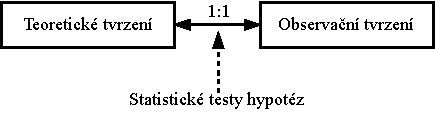
\includegraphics[width=.5\textwidth]{obrazky/GUHA/GUHA1.pdf}
    \caption{Vztah mezi tvrzeními vzorku dat a celých dat v metodě GUHA. Zdroj: vlastní.}
    \label{obr:met:GUHA1}
\end{figure}

Základní postup GUHA procedury je na obrázku \ref*{obr:met:GUHA2}. Vstupem pro procedury jsou vstupní data a parametry, které definují množinu relevantních tvrzení. Na základě definice jsou vytvořena všechna relevantní observační tvrzení, která jsou verifikována podle dat. Výstupem jsou pak všechna všechna prosté observační tvrzení vycházející ze vstupů. Prosté relevantní  tvrzení je takové tvrzení, které je pravdivé ve vstupních datech a zároveň neplyne již z uvedeného jiného tvrzení ve výstupu.\cite{bib:GUHA}

\begin{figure}[hbtp!]
    \centering
    \captionsetup{justification=centering}
    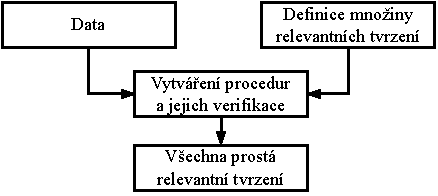
\includegraphics[width=.5\textwidth]{obrazky/GUHA/GUHA2.pdf}
    \caption{Základní postup procdury GUHA. Zdroj: vlastní.}
    \label{obr:met:GUHA2}
\end{figure}

\subsubsection{Důležité pojmy}


% Uvažujeme potenciálně nekonečnou množinu objektů. Metoda předpokládá výsledky existenci pozorování této množiny reprezentované v~matici dat. Cílem je získat všechny zajímavé vztahy, které jsou pravdové pro celou množinu objektů

Pro podrobnější popis procedur je nejprve třeba definovat několik pojmů, se kterými se v procedurách pracuje. Metoda pracuje s nádledujícími pojmy \cite{bib:GUHA}:

\begin{itemize}
    \itemsep0em
    \item \textbf{Matice dat a atributy} -- Řádky matice jsou jednotlivá pozorování. Atributem se rozumí sledovaná vlastnost, jedná se o sloupec matice.
    \item \textbf{Základní booleovský atribut} -- Jedná se o výraz $\bm{\mathrm{A(\alpha)}}$, kde $\bm{\mathrm{A}}$ je atribut a  $\bm{\alpha}$ je vlastní podmnožina $\bm{\mathrm{A}}$. $\bm{\alpha}$ může obsahovat více prvků než jeden.
    \item \textbf{Booleovský atribut} -- Každý základní boolovský atribut je booleovský atribut. Boolovské atributy jsou i negace, konjunkce a disjunkce základních boolovských atributů. 
    \item[] Pro každý řádek $i$ matice $\mathbf{M}$ nabývá boolovský atribut  $\bm{\mathrm{A}}$ hodnotu $0$, nebo $1$.
    \begin{equation*}
    \bm{\mathrm{A}}\left[i\right] = 1 \Rightarrow \mbox{boolovský atribut } \bm{\mathrm{A}} \mbox{ je pravdivý pro řádek } i.
    \end{equation*}
    \begin{equation*}
        \bm{\mathrm{A}}\left[i\right] = 0 \Rightarrow \mbox{boolovský atribut } \bm{\mathrm{A}} \mbox{ je nepravdivý pro řádek } i.
        \end{equation*}

    \item \textbf{Literál} -- Základní boolovský atribut nebo jeho negace.
    \item \textbf{Dílčí cedent} -- Konjunkce nebo disjunkce literálů.
    \item \textbf{Cedent} -- Jedná se o konjunkci dílčích cedentů. Příkladem cedentu je booleovský atribut, který vznikl konjunkcí a disjunkcí dalších atributů.

\end{itemize}


Další pojmy se týkají vztahů, se kterými procedury pracují \cite{bib:GUHA}:

\begin{itemize}
    \itemsep0em
    \item \textbf{Asociační pravidlo} -- Výraz $\mathrm{X} \rightarrow \mathrm{Y}$, kde $\mathrm{X}$ a $\mathrm{Y}$ jsou konjunkce dvojic atribut a jeho hodnota. Dále v textu je použivaná pro tento pojem zkratka AP.
    \item \textbf{Konfidence AP} -- Podíl počtu řádků, které splňují A a zároveň S a počtu řádků, které splňují pouze S.
    \item \textbf{Podpora AP} -- Podíl počtu řádků, které splňují A a zároveň S a počtu řádků vstupní matice dat.
\end{itemize}

Častou úlohou pro dobývání AP je nalezení všech AP, u kterých je hodnota konfidence a podpory AP větší nebo rovna danému prahu. V rámci GUHA se AP zkoumají jako vztah dvou obecných boolovských atributů, které jsou odvozené ze sloupců vstupní matice. GUHA asociační pravidlo (GUHA AP) je 
výraz 
\begin{equation}
    \varphi \approx \psi, 
\end{equation}
kde $\varphi, \psi$ jsou boolovské atributy, které nemají obsažený žádný společný boolovský atribut. $\varphi$ se nazývá \emph{antecedent} a $\phi$ \emph{sukcedent}\footnote{Antecedent, jako cedent, který předchází a sukcedent, jako cedent, který následuje.}. Symbol $\approx$ odpovídá \emph{4ft-kvantifikátoru}, viz dále v této sekci. Existují také podmíněná GUHA AP, která mají tvar  $\varphi \approx \psi | \chi$, kde $\chi$ je boolovský atribut.\cite{bib:GUHA}

Pravdivost GUHA AP v matici dat $\mathbf{M}$ se určuje pomocí tzv. \emph{4ft-tabulky}. Nechť je dána matice vstupních dat $\mathbf{M}$, antecedent $\varphi$, sukcedent $\psi$. Pak \emph{4ft-tabulka} $\mathrm{4ft}(\varphi,\psi,\mathbf{M})$ je definována jako čtveřice čísel $(a,b,c,d)$, pro které platí:
\begin{itemize}
    \itemsep0em
    \item $a$ je počet řádků matice $M$, které splňují oba boolovské atributy $\varphi, \psi$.
    \item $b$ je počet řádků matice $M$, které splňují $\varphi$, ale nesplňují $\psi$.
    \item $c$ je počet řádků matice $M$, které nesplňují $\varphi$, ale splňují $\psi$.
    \item $d$ je počet řádků matice $M$, které nesplňují ani jeden atribut $\varphi, \psi$.\cite{bib:GUHA}
\end{itemize}
Reprezentace této tabulky je zobrazena v tab. \ref*{tab:GUHA:tabulka}.

\begin{table}[hbtp!]
    \begin{center}
            \captionsetup{justification=centering}
    \caption{\emph{4ft-tabulka} matice $\mathbf{M}$ s asociačním pravidlem $\varphi \approx \psi$.}
    \begin{tabular}{c|c|c}
        $\mathbf{M}$ & $ \;\psi \;$& $\neg\,\psi$ \\
        \hline
        $\varphi$ & $a$& $b$ \\
        \hline
        $\neg\,\varphi$ & $c$& $d$ \\
        \end{tabular}
    \label{tab:GUHA:tabulka}
\end{center}
\end{table}

\emph{4ft-kvanitifikátor}, symbol $\approx$, definuje podmínku, která se týká hodnot $(a,b,c,d)$ v \emph{4ft-tabulce}. Kvantifikátor je formálně definovaný pomocí funkce $F_\approx$, která každé čtveřici nezáporných čísel přiřazuje hodnotu $1$, resp. $0$ pokud je, resp. není podmínka splněna. Zapisujeme $F_\approx(a,b,c,d)$ nebo zkráceně $\approx(a,b,c,d)$.\cite{bib:GUHA}
\begin{equation}
\begin{aligned}
    \mbox{GUHA AP } & \varphi \approx \psi \mbox{ je pravdivé v matici dat }\mathbf{M} \\
    & \Leftrightarrow \approx(a,b,c,d) = 1 \mbox{, formálně zapsáno jako } \mathrm{Val}(\varphi \approx \psi) = 1.   \\
    \vspace*{.5em} \\
    \mbox{GUHA AP } & \varphi \approx \psi \mbox{ je nepravdivé v matici dat }\mathbf{M} \\
   & \Leftrightarrow \approx(a,b,c,d) = 1 \mbox{, formálně zapsáno jako } \mathrm{Val}(\varphi \approx \psi) = 1. 
\end{aligned}
\end{equation}

Pro podmíněné AP $\varphi \approx \psi | \chi$ platí obdobné vztahy. Předpokládáme však, že boolovský atribut $\chi$ nemá ani jeden společný .atribut s atributy $\varphi$ a $\psi$. Platí tvrzení \cite{bib:GUHA}:
\begin{equation}
    \begin{aligned}
        &\mbox{Nechť } \mathbf{M} \mbox{ je matice vstupních dat, } \varphi,\psi,\chi  \mbox{ boolovské atributy, } \approx \mbox{ kvantifikátor.} \\
        & \mbox{Podmíněné AP } \varphi \approx \psi | \chi \; \mbox{je pravdivé v } \mathbf{M} \Leftrightarrow \varphi \approx \psi \; \mbox{ je pravdivé v matici } \mathbf{M|}\chi.
    \end{aligned}
\end{equation}

\subsubsection{Procedury}

V dokumentaci \cite{bib:GUHA} je popsáno sedm procedur -- \emph{4ft-Miner,  SD4ft-Miner, CF-Miner, SDCF-Miner,  KL-Miner,  SDKL-Miner,  Ac4ft-Miner} \cite{bib:GUHA}. V knihovně v jazyce Python jsou implementované pouze metody \emph{4ft-Miner, SD4ft-Miner, CF-Miner} \cite{bib:GUHAclever}. V této práci jsem použila metodu pouze první metodu, proto další je další teoretický popis věnován pouze metodě \emph{4ft-Miner}.

Tato procedura pracuje s AP $\varphi \approx \psi$, nebo s podmíněnými AP $\varphi \approx \psi | \chi$. V knihovně \emph{Cleverminer} lze v hlavní funkci \texttt{cleverminer} předat vstupní DataFrame s daty, který reprezentuje vstupní matici dat, další parametr je jedna ze tří implementovaných procedur, dále seznam podmínek pro vyhodnocení tvrzení, vypnutí optimalizace, limit pro výsledná tvrzení a seznam cedentů. Cedenty jsou rozděleny na antecedenty (parametr \texttt{ante}, tj. boolovský atribut $\varphi$), sukcedenty (parametr \texttt{succ}, tj. atribut $\psi$) a podmínky (parametr \texttt{cond}, tj. boolovský atribut $\chi$).
Každý z boolovských atributů libovolného typu cedentu může mít tyto atributy:
\begin{itemize}
    \itemsep0em
    \item \texttt{name} -- Název příznaku matice, tj. název sloupce v DataFramu.
    \item \texttt{type} -- Jakým pravidlem se řídí výběr více kategorií v příznaku. Jedna z hodnot \texttt{subset, lcut, rcut, seq, one}. 
    \item \texttt{minlen} -- Minimální počet kategorií v daném příznaku.
    \item \texttt{maxlen} -- Maximální počet kategorií v daném příznaku.\cite{bib:GUHAclever}
\end{itemize}

Příznaky musí být kategorické a musí být možné je seřadit. Druhá vlastnost je třeba pro vybírání více kategorií v jednom cedentu určitými způsoby selekce. Pro textové řetězce reprezentující kategorie jsou názvy kategorií řazeny podle abecedy.\cite{bib:GUHAclever}

Pro názornost jsou dále uvedeny příklady pro jednotlivé druhy atributu \texttt{type}. Nechť je dán příznak $\mathbf{A}$ s kategoriemi 1, 2, 3, 4, 5 a parametry jsou definovány následovně: \texttt{minlen=1}, \texttt{minlen=3}. Pokud je typ \texttt{one}, bere se jedna z kategorií daného příznaku, tuto kategorii je třeba specifikovat. Pro typ \texttt{subset} jsou vybrány všechny následující možnosti:
\begin{itemize}
    \itemsep0em
    \item Délka je rovna 1 --  $\mathbf{A(1), A(2), A(3), A(4), A(5)}.$
    \item Délka je rovna 2 --  $\mathbf{A(1, 2), A(1, 3), A(1, 4), A(1, 5), A(2, 3), A(2, 4), A(2, 5)},$
    \item[] $\mathbf{A(3, 4), A(3, 5), A(4, 5)}.$
    \item Délka je rovna 3 --  $\mathbf{A(1, 2, 3), A(1, 2, 4), A(1, 2, 5),A(2, 3, 4), A(2, 3, 5),}$
    \item[] $\mathbf{A(3, 4, 5)}$.\cite{bib:GUHA}
\end{itemize}
Pro typ sekvence, \texttt{seq} by se pak vybraly následující možnosti:
\begin{itemize}
    \itemsep0em
    \item Délka je rovna 1 --  $\mathbf{A(1), A(2), A(3), A(4), A(5)}.$
    \item Délka je rovna 2 --  $\mathbf{A(1, 2), A(2, 3), A(3, 4), A(4, 5)}.$
    \item Délka je rovna 3 --  $\mathbf{A(1, 2, 3), A(2, 3, 4), A(3, 4, 5)}$.\cite{bib:GUHA}
\end{itemize}

Pro typ \texttt{lcut} se vybírají možnosti:
\begin{itemize}
    \itemsep0em
    \item Délka je rovna 1 --  $\mathbf{A(1)}.$
    \item Délka je rovna 2 --  $\mathbf{A(1, 2)}.$
    \item Délka je rovna 3 --  $\mathbf{A(1, 2, 3)}$.\cite{bib:GUHA}
\end{itemize}
Analogicky pro typ \texttt{rcut}.

Literály v rámci cedentů lze také kombinovat obdobnými způsoby. Opět lze přiřa-\\dit minimální a maximální délku, typ pro kombinování literálů je výběr konjunkce, nebo disjunkce. Tyto možnosti lze specifikovat pro antecedenty, sukcedenty i pod-\\mínky. Zadání podmínek není nezbytné v atributech funkce \texttt{cleverminer}.

Další parametry, které lze předat této funkci jsou:
\begin{itemize}
    \itemsep0em
    \item \texttt{Base} -- Minimální počet řádků, které splňují antecedenty i sukcedenty (číslo $a$ v tabulce \ref*{tab:GUHA:tabulka}).
    \item \texttt{RelBase} -- Hodnota Base vydělená celkovým počtem řádků dat (případně počtem řádků v matici s aplikovanou podmínkou).
    \item \texttt{conf} -- Konfidence, pravděpodobnost $/mathrm{P}(\psi|\varphi)$. Jinými slovy procen--\\tuální zastoupení řádků, které vyhovují $\psi$ (sukcendentům) z těch řádků, které vyhovují i $\varphi$ (antecendtům).
    \item \texttt{aad} (nadprůměrná závislost) -- Jak moc $\varphi$ zvyšuje  pravděpodobnost $\psi$. Kolikrát se zvýší pravděpodobnost splnění sukcedentů, když se vezmou pouze záznamy, které vyhovují antecentům, oproti všem záznamům minus 1.
    \item \texttt{bad} (podprůměrná závislost) -- Jak moc $\varphi$ snižuje  pravděpodobnost $\psi$.
\end{itemize}

Příklad volání funkce \texttt{cleverminer} je sepsaný v ukázce kódu č. \ref*{code:cleverminer}.
\begin{lstlisting}[language=Python, style=mystyle, label={code:cleverminer}, caption={Příklad volání funkce \texttt{cleverminer}.}]
cleverminer(df = data,
            proc = "4ftMiner", 
            quantifiers = {"conf":0.6, "Base":1000},
            ante = {
                    "attributes":
                    [
                        {
                            "name":"weekday", 
                            "type":"subset", 
                            "minlen":1, "maxlen":3
                        },
                        {
                            "name":"quarter", 
                            "type":"lcut", 
                            "minlen":1, "maxlen":4
                        }
                    ], 
                    "minlen":1, "maxlen":3, "type":"con"
                    },
            succ = {
                    "attributes":
                    [
                        {
                            "name":"L3", 
                            "type":"subset", 
                            "minlen":1, "maxlen":3
                        }
                    ], 
                    "minlen":1, "maxlen":1, "type":"con"
                    },
            cond = {
                    "attributes":
                    [
                        {
                            "name":"promo", 
                            "type":"one", 
                            "value":"promo"
                        }
                    ],
                    "minlen":1, "maxlen":1, "type":"con"
                    }
            )
\end{lstlisting}


% \subsection{Genetický algoritmus}

% Genetický algoritmus byl inspirovaný evoluční teorií a přirozeným výběrem. Je založený na teorii, že jedinci, kteří jsou lepší než ostatní mají větší šanci na to, předat svou genetickou informaci dál. Jejich geny tk budou základem nové generace. Podobně jako ve zmíněné teorii, algoritmus používá následující informace: genetickou reprezentaci pomocí bitového  řetězce, funkci pro vyhodnocení tzv. fitness funkci, kombinování genů a mutaci. 

% Nejprve se vytvoří náhodná populace. Od této inicializační populace se postupně se iteruje dokud již další změny nevedou k~lepšímu řešení, nebo dokud neskončí počet iterací. Jedna iterace je analogií k~jedné evoluční generaci.

% Bitový řetězec populace se vyhodnotí pomocí cílové funkce (objective function). Hodnota cílové funkce pak určuje hodnotu fitness daného řešení. Fitness je možné uvažovat jako minimalizační nebo maximalizační kritérium.

% Dále se vyberou dva rodiče podle své fitness hodnoty, kteří se mezi sebou zkříží a jejich potomek vstoupí do další iterace. Jeden ze způsobů výběru je vybrat k~náhodných populací a znich vybrat populaci s nejvyšším fitness. Křížení rodičů je pravděpodobnostní, takže v~některých případech ,ůže vzniknout potomek stejný jako jeho rodič. Obvykle se hyperparametr pro křížení se nastavuje na vyšší hodnoty např. 80 nebo 90 \%. Dalším parametrem je mutace, ta určuje zda přenesený bit zmutuje nebo ne. Jeho hodnota se nastavuje jako $1/L$, kde $L$ je délka řetězce.



